%%%%%%%%%%%%%%%%%%%%%%%%%%%%%%%%%%%%%%%%%%%%%%%%%%%%%%%%%%%%%%%%%%%%%%%%%%%%%%%%
\chapter{Αποτελέσματα}

%%%%%%%%%%%%%%%%%%%%%%%%%%%%%%%%%%%%%%%%%%%%%%%%%%%%%%%%%%%%%%%%%%%%%%%%%%%%%%%%
\section{Καταγραφή της Κίνησης}

Ως αποτελέσματα της καταγραφής της κίνησης επιλέχθηκε αρχικά να παρουσιαστεί η ικανότητα καταγραφής του μήκους των τμημάτων του σώματος του ανθρώπου. Στο πείραμα συμμετείχαν δύο δείγματα τα οποία εκτέλεσαν διαφορετικές κινήσεις, όπου για κάθε κίνηση υπολογίστηκα το μέσο μήκος για κάθε τμήμα. Αφού συγκεντρώθηκαν τα αποτελέσματα κατασκευάστηκαν τα αντίστοιχα διαγράμματα που δείχνουν το μέσο μήκος για όλες τις καταγεγραμμένες κινήσεις, για κάθε τμήμα, μαζί με τις τυπικές αποκλίσεις.

\begin{figure}[H]
    \centering
    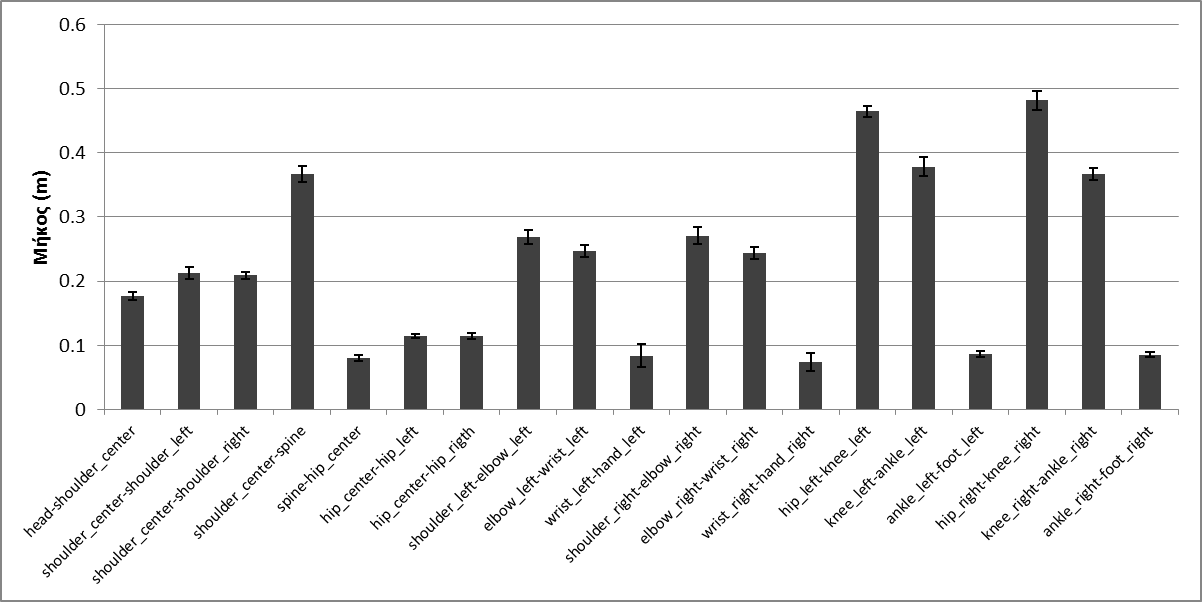
\includegraphics[width=.9\textwidth]{fig/subject01-segments.png}
    \caption{Μήκη τμημάτων για το πρώτο δείγμα (14 κινήσεις)}
    \label{fig:subject01-segments}
\end{figure}

Παρατηρούμε ότι οι τυπικές αποκλίσεις είναι μικρές με ελάχιστη για το πρώτο δείγμα στα $std_{min} = 0.0030m$ και με μέγιστη τιμή στα $std_{max} = 0.0182m$ \ref{fig:subject01-segments}. Όσον αφορά το δεύτερο δείγμα οι αντίστοιχες τυπικές αποκλίσεις είναι $std_{min} = 0.0.0019m$, $std_{max} = 0.0146m$ αντίστοιχα \ref{fig:subject02-segments}.

\begin{figure}[H]
    \centering
    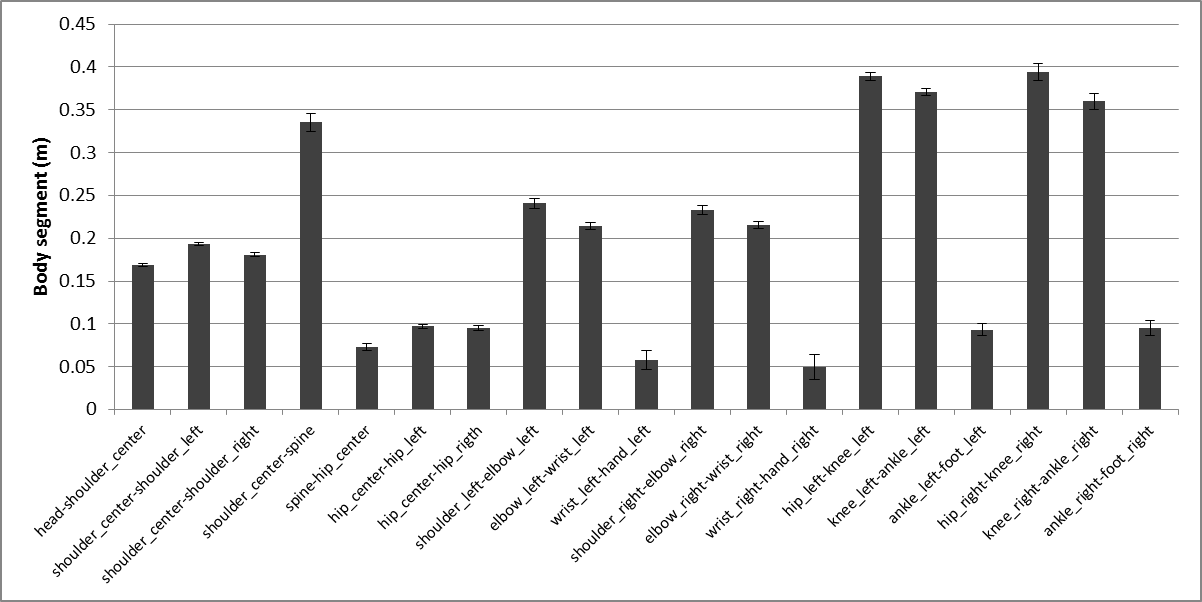
\includegraphics[width=.9\textwidth]{fig/subject02-segments.png}
    \caption{Μήκη τμημάτων για το δεύτερο δείγμα (5 κινήσεις)}
    \label{fig:subject02-segments}
\end{figure}

Ως δεύτερη σύγκριση του συστήματος, καταγράφτηκε μια κίνηση χωρίς την χρήση κάποιου φίλτρου και στην συνέχει καταγράφτηκε όμοια κίνηση με χρήση φίλτρου και ως παράμετροι επιλέχθηκαν οι τιμές για δυνατό φιλτράρισμα από τον πίνακα \ref{tab:filter-parameters}. Επίσης έγινε μια απλή υλοποίηση ενός φίλτρου \eng{Kalman} με βάση την εξής αναδρομική σχέση \ref{equ:kalman-predict-update} και επιλέχθηκαν τιμές για τα $R = 0.05,\; Q = 0.05$. Στον πίνακα \ref{tab:no-filter-filter-kalman} στην αριστερή στήλη είναι οι συντεταγμένες του δεξιού χεριού χωρίς την χρήση φιλτραρίσματος, ενώ δεξιά με χρήση φίλτρου. Με διακεκομμένες γραμμές φαίνεται η απόκριση του φίλτρου \eng{Kalman}. Στην περίπτωση που εκτελούμε φιλτράρισμα με δυνατό φίλτρο δεν διακρίνεται βελτιώσω από την χρήση του φίλτρου \eng{Kalman}, όπως έχει υλοποιηθεί. Φαίνεται όμως η ανάγκη για εξομάλυνση, οπότε απλά φίλτρα που φιλτράρουν τις απότομες μεταβολές βελτιώνουν πολύ το αποτέλεσμα.

\begin{equation}
    \begin{gathered}
        \text{Πρόβλεψη} \\
        \hat{p}_{t} = p_{t-1} + u_{t}, \quad u_{t} = \frac{p_{t-1} - p_{t-2}}{t_{t-1} - t_{t-2}} \\
        \hat{P} = P_{t-1} + Q \\[.5cm]
        \text{Διόρθωση} \\
        Κ = \frac{\hat{P}}{\hat{P} + R}\\
        p_{t} = \hat{p}_{t} + K \cdot (p_{t} - \hat{p}_{t}) \\
        P_{t} = (1 - K) \cdot \hat{P}
    \end{gathered}
    \label{equ:kalman-predict-update}
\end{equation}

\begin{center}
    \begin{tabular}{cc}
        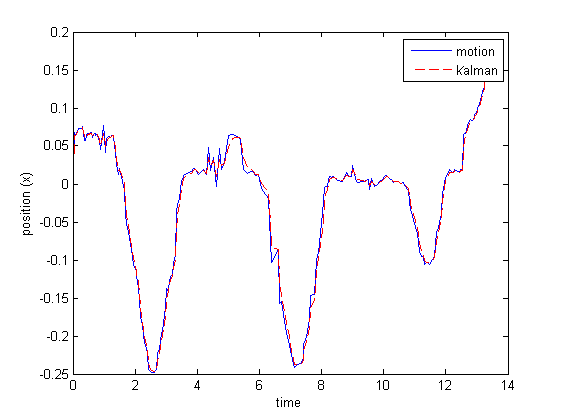
\includegraphics[width=.5\textwidth, height = 0.23\textheight, keepaspectratio]{fig/filter0-x.png} & 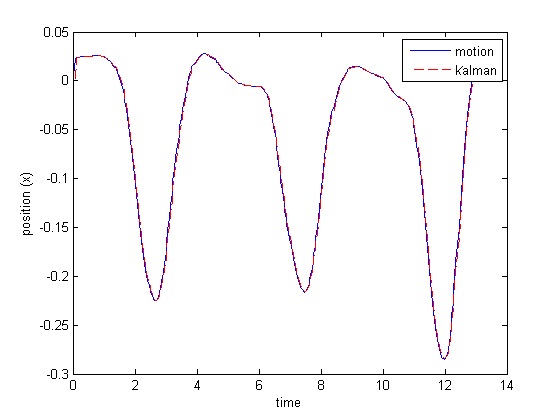
\includegraphics[width=.5\textwidth, height = 0.23\textheight, keepaspectratio]{fig/filter3-x.png}\\
        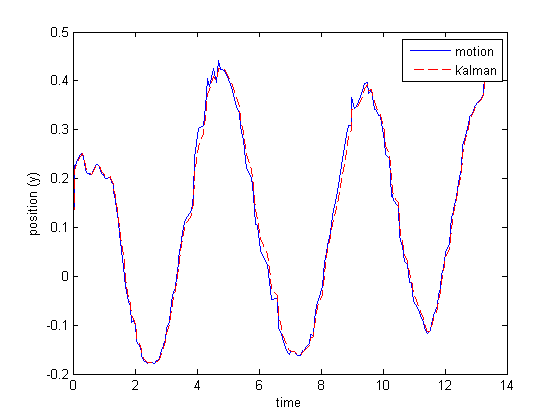
\includegraphics[width=.5\textwidth, height = 0.23\textheight, keepaspectratio]{fig/filter0-y.png} & 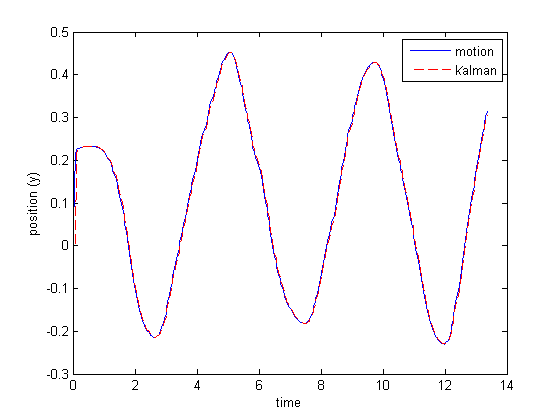
\includegraphics[width=.5\textwidth, height = 0.23\textheight, keepaspectratio]{fig/filter3-y.png}\\
        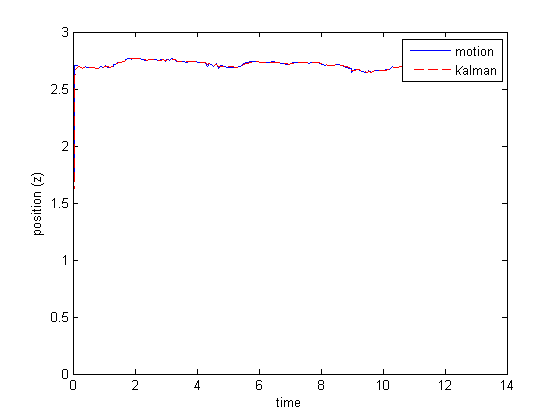
\includegraphics[width=.5\textwidth, height = 0.23\textheight, keepaspectratio]{fig/filter0-z.png} & 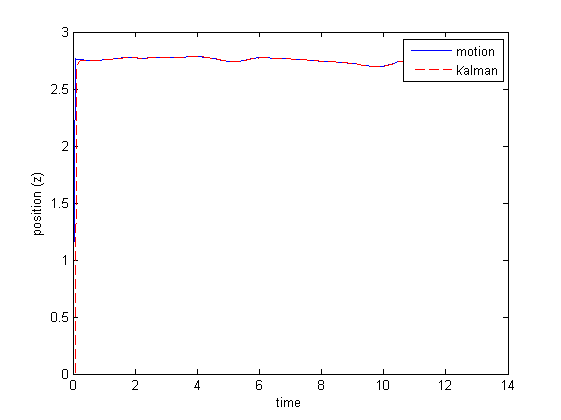
\includegraphics[width=.5\textwidth, height = 0.23\textheight, keepaspectratio]{fig/filter3-z.png}\\
        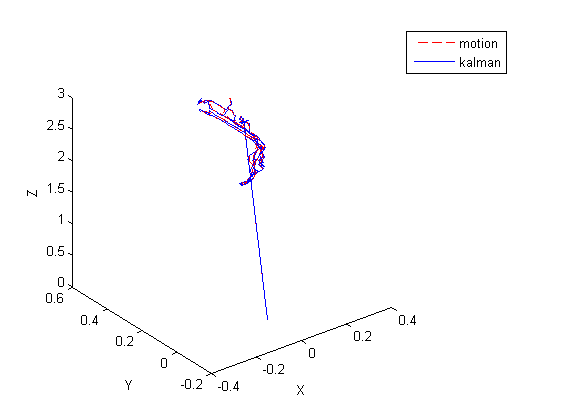
\includegraphics[width=.5\textwidth, height = 0.23\textheight, keepaspectratio]{fig/filter0-xyz.png} & 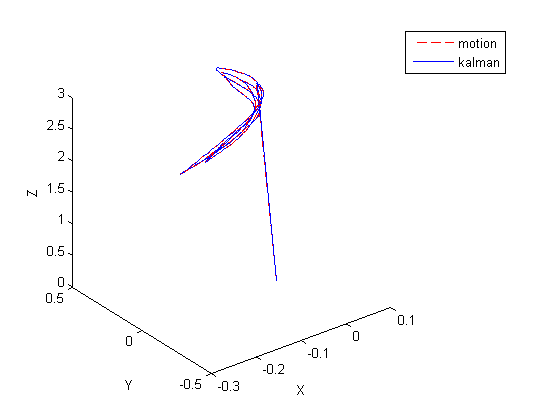
\includegraphics[width=.5\textwidth, height = 0.23\textheight, keepaspectratio]{fig/filter3-xyz.png}
    \end{tabular}
    \captionof{table}{Συντεταγμένες του δεξιού χεριού χωρίς φιλτράρισμα αριστερά και με φιλτράρισμα δεξιά}
    \label{tab:no-filter-filter-kalman}
\end{center}
%%%%%%%%%%%%%%%%%%%%%%%%%%%%%%%%%%%%%%%%%%%%%%%%%%%%%%%%%%%%%%%%%%%%%%%%%%%%%%%%
\section{Αντίστροφη Κινηματική}

Για να υπάρχουν σωστά αποτελέσματα κατά την αντίστροφη κινηματική είναι αναγκαία η διαδικασία της κανονικοποίησης ώστε το γενικό μοντέλο να πάρει τις διαστάσεις του δείγματος. Οπότε η διαδικασία της κανονικοποίησης θεωρείται δεδομένη κάθε φορά. Αυτό που μπορούμε να εκθέσουμε ως αποτέλεσμα της διαδικασίας είναι το σφάλμα της αντίστροφης κινηματικής. Για το πείραμα εκτελέστηκε η αντίστροφη κινηματική για 6 διαφορετικές κινήσεις του ίδιου δείγματος και καταγράφηκε το συνολικό τετραγωνικό σφάλμα (\eng{total square error}), το σφάλμα λόγω ενδείξεων (\eng{marker error}) και το μέγιστο σφάλμα από όλες τις αρθρώσεις (\eng{max joint error}). Τα τρία αυτά σφάλματα ήταν διαθέσιμα για κάθε χρονική στιγμή που υπολογίζονταν η αντίστροφη κινηματική. Ως εκ τούτο για κάθε ένα από αυτά τα σφάλματα υπολογίστηκε η μέση τιμή, η τυπική απόκλιση και η μέγιστη τιμή από όλες τις χρονικές στιγμές για κάθε κίνηση ξεχωριστά.

\begin{center}
    \begin{tabular}{cc}
        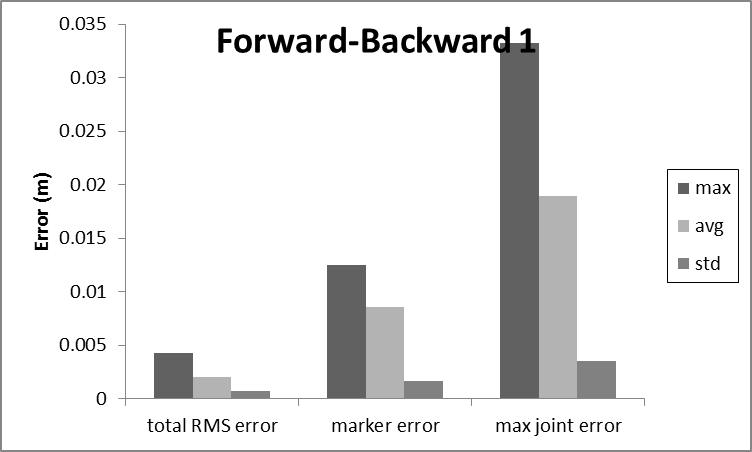
\includegraphics[width=.48\textwidth, keepaspectratio]{fig/ik-reg1.png} & 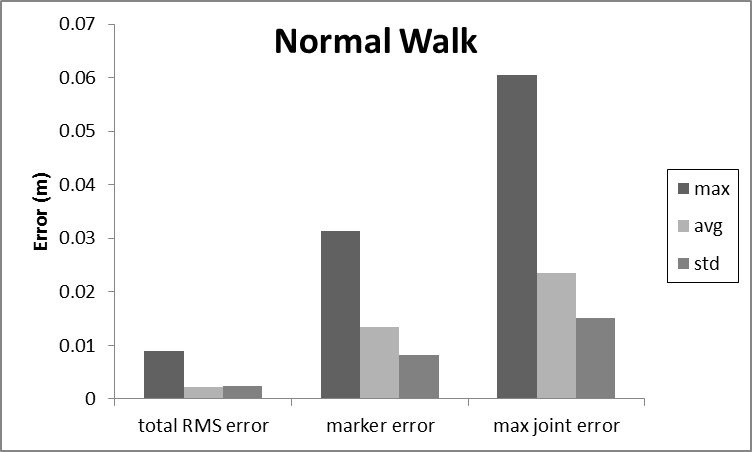
\includegraphics[width=.48\textwidth, keepaspectratio]{fig/ik-reg2.png}\\[3pt]
        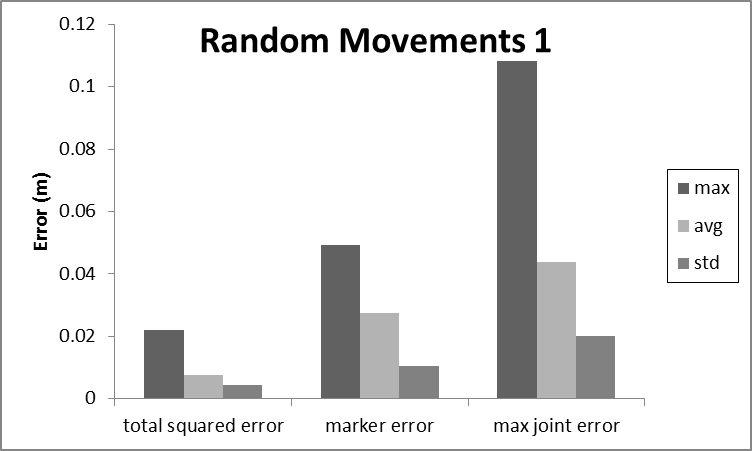
\includegraphics[width=.48\textwidth, keepaspectratio]{fig/ik-reg3.png} & 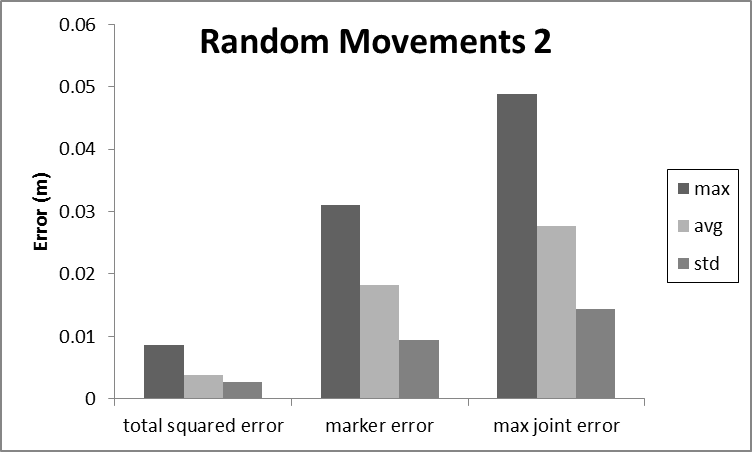
\includegraphics[width=.48\textwidth, keepaspectratio]{fig/ik-reg4.png}\\[3pt]
        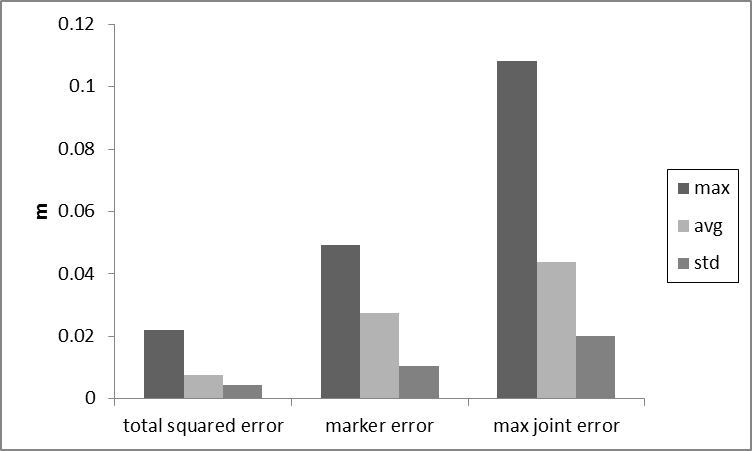
\includegraphics[width=.48\textwidth, keepaspectratio]{fig/ik-reg5.png} & 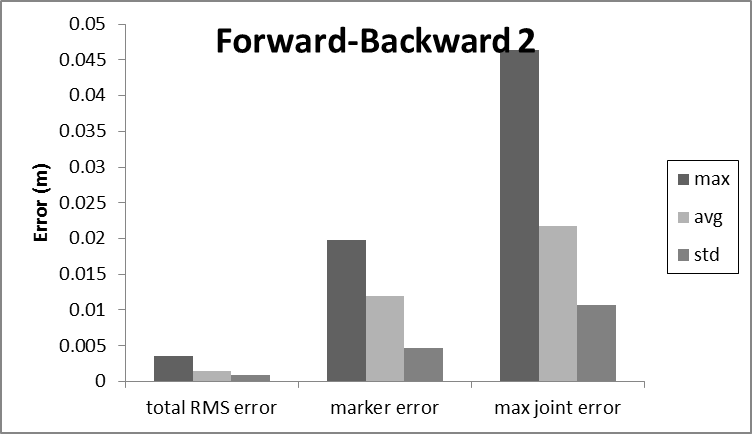
\includegraphics[width=.48\textwidth, keepaspectratio]{fig/ik-reg6.png}
    \end{tabular}
    \captionof{table}{Τα σφάλματα της αντίστροφης κινηματικής ανά περιοχή}
    \label{tab:ik-error-regions}
\end{center}

%%%%%%%%%%%%%%%%%%%%%%%%%%%%%%%%%%%%%%%%%%%%%%%%%%%%%%%%%%%%%%%%%%%%%%%%%%%%%%%%
\section{Αντίστροφη Δυναμική}

Με την αντίστροφη δυναμική έχουμε στην διάθεση μας τις ροπές που ασκούνται στις αρθρώσεις κάθε χρονική στιγμή. Λόγο της δυσκολίας υπολογισμού των εξωτερικών δυνάμεων, χρησιμοποιήθηκαν δεδομένα βάδισης και καταγεγραμμένη αντίδραση εδάφους που βρέθηκε στο διαδίκτυο, ώστε να επιβεβαιωθεί η ισχύς της ανάλυσης. Στην μελέτη των ροπών, παρουσιάζονται η ροπές του γοφού, του γονάτου και του αστράγαλου σε ένα κύκλο βάδισης και συγκρίνονται με την βιβλιογραφία \cite{whittlesey}. Στον πίνακα \ref{tab:id-hip-knee-ankle-moments} από αριστερά είναι οι πειραματικές ροπές για έναν κύκλο βάδισης για τον γοφό, το γόνατο και τον αστράγαλο και από δεξιά είναι τα αντίστοιχα με βάση την βιβλιογραφία. Τα δικά μας διαγράμματα είναι ανάποδα γιατί έχουμε θεωρήσει διαφορετικές φορές, ωστόσο συμβαδίζουν τα αποτελέσματα μας με βάση την βιβλιογραφία αν λάβουμε υπόψιν τις ενδείξεις πάνω στα διαγράμματα.

\begin{center}
    \begin{tabular}{cc}
        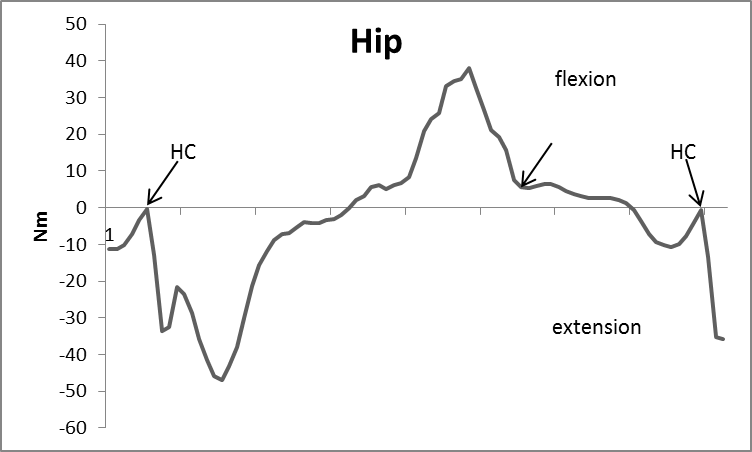
\includegraphics[width=.48\textwidth, keepaspectratio]{fig/id-hip.png} & 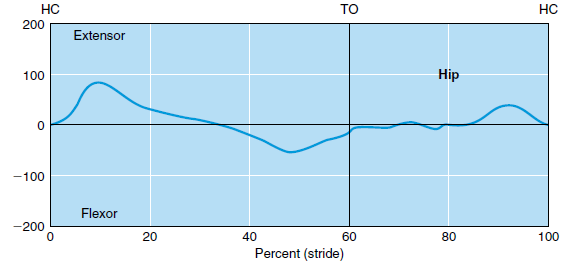
\includegraphics[width=.48\textwidth, keepaspectratio]{fig/id-hip-ref.png}\\[3pt]
        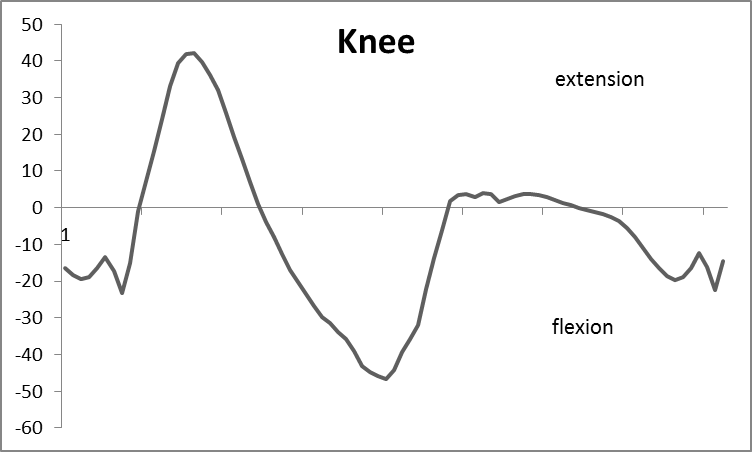
\includegraphics[width=.48\textwidth, keepaspectratio]{fig/id-knee.png} & 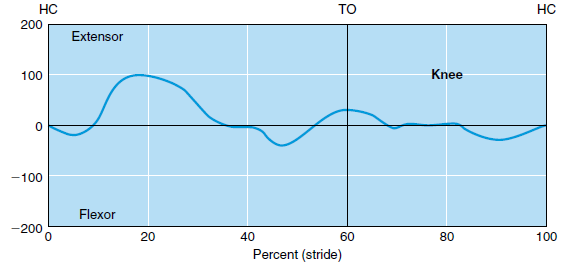
\includegraphics[width=.48\textwidth, keepaspectratio]{fig/id-knee-ref.png}\\[3pt]
        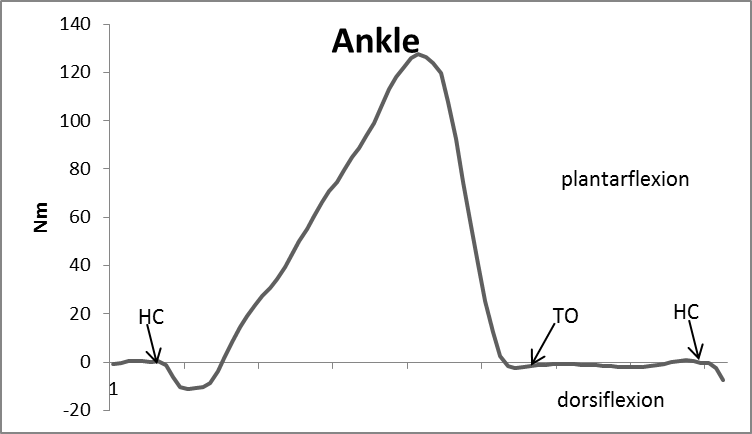
\includegraphics[width=.48\textwidth, keepaspectratio]{fig/id-ankle.png} & 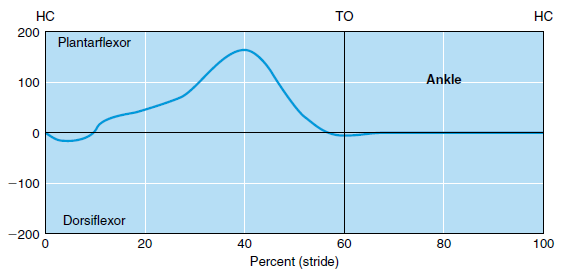
\includegraphics[width=.48\textwidth, keepaspectratio]{fig/id-ankle-ref.png}
    \end{tabular}
    \captionof{table}{Σύγκριση ροπής για ένα κύκλο βάδισης}
    \label{tab:id-hip-knee-ankle-moments}
\end{center}
